\documentclass[
	12pt,
	a4paper,
	BCOR10mm,
	%chapterprefix,
	DIV14,
	listof=totoc,
	bibliography=totoc,
	headsepline
]{scrreprt}

% Encoding Options
\usepackage[T1]{fontenc}
\usepackage[utf8]{inputenc}
% Language
\usepackage[english]{babel}

% BibLaTex incl. Biber as backend
\usepackage[
	% General options
	backend=biber,
	style=alphabetic,
	sortlocale=en_US,
	% Specific options
	% backref=true,
	doi=true,
	eprint=false,
	hyperref=true,
	url=true]{biblatex}
\addbibresource{sources.bib}

% change date format from 'mm/dd/yyyy' to 'dd. mm . yyyy' TODO: revert later?
\renewbibmacro*{url+urldate}{%
\printfield{url}%
\iffieldundef{urlyear}
	{}
	{\setunit*{\addspace}%
	\printtext[urldate]{\printfield{urlday}\setunit*{\adddot\addthinspace}%
			\printfield{urlmonth}\setunit*{\adddot\addthinspace}%
			\printfield{urlyear}%\setunit*{\adddot}
}}}%

\addto\captionsenglish{% Replace "english" with the language you use
	\renewcommand{\contentsname}{Table of Contents}
}

% Modern latin font
\usepackage{lmodern}

% Load xcolor first
\usepackage[usenames, dvipsnames]{xcolor}

% Various useful packages
\usepackage[footnote]{acronym}
\usepackage[page]{appendix}
\usepackage{booktabs}
\usepackage{caption}
\usepackage[autostyle,babel,strict]{csquotes}
\usepackage{footnote}
\usepackage{float}
\usepackage{graphicx}
\usepackage[htt]{hyphenat}
\usepackage{listings}
\usepackage{microtype}
\usepackage{pdflscape}
\usepackage{pgfplots}
\usepackage{scrlayer-scrpage}
\usepackage{subfig}
\usepackage{textcomp}
\usepackage{tikz}
\usepackage{tikzscale}
\usepackage[subfigure,titles]{tocloft}
\usepackage{units}
\usepackage{xparse}

% For dates
\newcommand{\leadingzero}[1]{\ifnum #1<10 0\the#1\else\the#1\fi}

% Allow footnotes in tables
\makesavenoteenv{tabular}
\makesavenoteenv{table}

% Use hyperref last to make sure it can define all necessary commands
\usepackage[pdfborder={0 0 0}]{hyperref}

\addto\extrasenglish{%
	\def\chapterautorefname{Chapter}%
	\def\sectionautorefname{Section}%
}

% Use glossaries/xindy after hyperref to make it use links
\usepackage[nonumberlist,nopostdot,numberedsection=autolabel,style=altlist,toc,xindy]{glossaries}
\usepackage[xindy]{imakeidx}

% Command to create dual entries (acronyms with description)
\DeclareDocumentCommand{\newdualentry}{ O{} O{} m m m m } {
  \newglossaryentry{gls-#3}{name={#5},text={#5\glsadd{#3}},
    description={#6},#1
  }
  \newacronym[see={[Glossary:]{gls-#3}},#2]{#3}{#4}{#5\glsadd{gls-#3}}
}

% Setup glossaries
\loadglsentries[main]{misc/glossary}
\makeglossaries
\makeindex
% \renewcommand*{\glsautoprefix}{ap:gl_}

% Limit ToC depth
\setcounter{tocdepth}{1}

% Page (indent) definitions
\sloppy
\setlength{\parindent}{0em}
\setlength{\parskip}{1.2ex plus 0.5ex minus 0.5ex}

% Some pdf related meta-information
\hypersetup{
	pdftitle	={Evaluation of performance and productivity metrics of potential programming languages in the HPC environment},
	pdfauthor 	={Florian Wilkens},
	pdfkeywords ={HPC, Rust, C, Go, performance, productivity}
}

% Set default graphicspath to 'img' folder
\graphicspath{img}

% Define some custom colors
\definecolor{light-gray}{gray}{0.85}
\definecolor{comment-green}{HTML}{009900}

% Define language environments or listings
\lstdefinestyle{base}{
	basicstyle=\ttfamily,
	breakatwhitespace=true,
	breaklines=true,
	captionpos=b,
	commentstyle=\color{comment-green},
	frame=single,
	keywordstyle=\color{blue},
	numbers=left,
	numberstyle=\tiny,
	rulecolor=\color{black},
	% prebreak=\textbackslash,
	postbreak=\hbox{$\hookrightarrow$ },
	showstringspaces=false,
	stringstyle=\color{red},
	tabsize=4
}

\lstdefinestyle{plain}{
	style=base,
	numbers=none
}

\lstdefinestyle{shell}{
	style=plain
	%language=sh
}

\lstdefinestyle{c}{
	language=C,
	style=base,
	morekeywords={pragma, omp}
}

\lstdefinestyle{go}{
	language=C,
	style=base,
	morekeywords={func, type, import, go, make, package, uint, int8, uint8, int16, uint16, int32, uint32, int64, uint64, float32, float64}
}

\lstdefinestyle{rust}{
	language=C,
	style=base,
	morekeywords={fn, let, self, match, move, mut, in, use, i8, u8, i16, u16, i32, u32, i64, u64, isize, usize, f32, f64, Vec},
	stringstyle=\color{black}
}

\lstdefinestyle{python}{
	language=python,
	style=base
}

\lstdefinestyle{erlang}{
	language=erlang,
	style=base,
	morekeywords={MODULE}
}

% Define some custom commands for inlining code, file names or shell commands
\newcommand{\mdinline}[1]{\colorbox{light-gray}{\texttt{#1}}}
\newcommand{\shinline}[1]{\textbf{\texttt{#1}}}

% Custom footnote command that adds \hspace before the text
\newcommand{\fnote}[1]{\footnote{\hspace{2pt}#1}}

% Change name of listing from 'Listings' to 'List of Listings' to be consistent
\renewcommand*{\lstlistlistingname}{List of Listings}

% Change abstract command to something useful
\renewcommand{\abstract}[1]{\textit{#1}\bigskip}

\begin{document}

\begin{titlepage}
    \begin{center}
        {\titlefont\huge Evaluation of performance and productivity metrics of
            potential programming languages in the HPC environment \par}

        \bigskip
        \bigskip

        {\titlefont\Large --- Bachelor Thesis ---\par}

        \bigskip
        \bigskip

        {\large Research group Scientific Computing \\
        Department of Informatics \\
        Faculty of Mathematics, Informatics und Natural Sciences \\
        University of Hamburg\par}
    \end{center}

    \vfill

    {\large \begin{tabular}{ll}
        Submitted by: & Florian Wilkens \\
        E-Mail: & \href{mailto:1wilkens@informatik.uni-hamburg.de}
            {1wilkens@informatik.uni-hamburg.de} \\
        Matriculation number: & 6324030 \\
        Course of studies: & Software-System-Entwicklung \\
        \\
        First assessor: & Prof. Dr. Thomas Ludwig \\
        Second assessor: & Sandra Schr\"oder \\ \\
        Advisor: & Michael Kuhn, Sandra Schr\"oder \\
        \\
        Hamburg, \today
    \end{tabular}\par}
\end{titlepage}


\chapter*{Abstract}

\thispagestyle{empty}

This thesis aims to analyze new programming languages in the context of HPC. To compare not only speed
but also development productivity and general inner metrics, a basic traffic simulation is implemented
in C, Mozilla's Rust and Google's Go. These two languages were chosen on their basic promise of
performance as well as memory-safety in the case of Rust or easy multhithreaded execution (Go).
The implementations are limited to shared-memory parallelism to achieve a fair comparison since the
library support for inter-process communication is rather limited at the moment.
\\
Nonetheless the comparison should allow a decent rating of the viability of these two languages in
high-performance computing.

% Really use company names?
% Last sentence is not symmetrical between languages


\microtypesetup{protrusion=false} % disable protrusion locally for the toc
\tableofcontents 				  % prints Table of Contents
\microtypesetup{protrusion=true}  % reenable protrusion

\chapter{Introduction}
\label{ch:Introduction}

\abstract{This chapter provides some background information to \gls{hpc}. The first section describes problems with the currently used programming languages and motivates the search for new candidates. After that the chapter concludes with a quick rundown of the thesis' goals.
}

\section{Motivation}
\label{sec:Introduction::Motivation}

The world of \acrlong{hpc} is evolving rapidly and programming languages used in this environment are held up to a very high performance standard. This is not surprising when an hour of computation costs thousands of dollars~\cite{cost_of_science}. The focus on raw power led to C and Fortran having an almost monopolistic position in the field, because their execution speed is nearly unmatched.

However programming in these rather antique languages can be rather difficult. Although they are still in active development, their long lifespans resulted in sometimes unintuitive syntax accumulated over the past centuries. Especially C's \textit{undefined behavior} often causes inexperienced programmers to write unreliable code which is unnecessarily dependent on implementation details of a specific compiler or the underlying machine. Understanding and maintaining these programs requires deep knowledge of memory layout and other technical details. In contrast Fortran does not require the same amount of technical knowledge but also limits the programmer in fine grained resource control. Both approaches are not ideal and the situation could be improved by a language offering both control and high-level abstractions while keeping up with Fortran and C's execution performance.

Also considering the fact that scientific applications are often written by scientist without a strong background in computer science it is evident that the current situation is less than ideal. There have been various efforts to make programming languages more accessible in the recent years but unfortunately none of the newly emerged ones have been successful in establishing themselves in the \gls{hpc} community to this day. Although many features and concepts have found their way in newer revision of C and Fortran standards most of them feel tacked on and are not well integrated into the core language.

One example for this is the common practice of testing. Specifically with the growing popularity of \textit{\gls{tdd}} it became vital to the development process to be able to quickly and regularly execute a set of tests to verify growing implementations as they are developed. Of course there are also testing frameworks and libraries for Fortran and C but since these languages lack deep integration of testing concepts, they often require a lot of setup and boilerplate code lowering developer productivity. In contrast, for example, the Go programming language includes a complete testing framework with the ability to perform benchmarks, perform global setup/tear-down work and even do basic output verification~\cite{go_doc_testing}.

While testing is just one example there are a lot of ``best practices'' and techniques which can greatly increase both developer productivity and code quality but require a language-level integration to work best. Combined with the advancements in type system theory and compiler construction both C and Fortran's feature sets look very dated. With this in mind it is time to review new potential successors of the two giants of \gls{hpc}.

\section{Goals of this Thesis}
\label{sec:Introduction::Goals}

This thesis aims to evaluate Rust and Go as potential programming languages in the \gls{hpc} environment. The comparison is based on three implementations of a shortest path algorithm in the two language candidates as well as C. The idea is based on an existing parallel application called \textit{streets4MPI} which was written in Python. It simulates ongoing traffic in a geographical area creating heat-maps as a result. The programs written for this thesis implement the computational intensive part which is the shortest path calculation to be able to review Go and Rust's performance characteristics as well as development productivity based on multiple criteria. Since libraries for inter-process communication in Rust and Go are nowhere near production-ready this thesis will focus on shared memory parallelization. Additionally unfair bias based solely on the quality of the supporting library ecosystem should be avoided.

To reduce complexity the implementations perform no real error handling nor produce any usable simulation output. They simply perform Dijkstra's algorithm in the most language idiomatic way which can optionally be parallelized. While raw performance will be the main criteria, additional productivity metrics will also be reviewed to rate the general development experience. Another focus will be the barrier of entry for newcomers to the respective languages which is important for scientist less proficient in programming.

\section{Structure}
\label{sec:Introduction::Structure}

This first chapter briefly motivated the search for new languages in \gls{hpc} and outlined the goals of the thesis. The second chapter \textit{State of the Art} describes common programming paradigms in C and Fortran and introduces the various languages which were considered for further evaluation. The following chapter \textit{Concept} describes the original case study \textit{streets4MPI} which the evaluation is based on, illustrates the various phases of the implementation process and mentions some related work. The fourth chapter \textit{Implementation} describes each implementation milestone in detail providing and briefly comparing intermediate results. The fifth chapter \textit{Evaluation} compares the various criteria for both performance and productivity and judges them accordingly. The final chapter \textit{Conclusion} summarizes the results of the evaluation and lists some possible improvements and future work.


\chapter{State of the art}
\label{chap:State_of_the_art}

\abstract{%
This chapter describes the current state of the art in high-performance computing. The dominance of Fortran and C is explained and questioned in~\autoref{sec:State_of_the_art::Paradigms}. After that all considered language candidates are introduced and characterized.
}

- state of C and Fortran (section name?)

- technological advancements in low level languages
    - static analysis
    - ..
    -> But no real adaption possible, because language level support is missing (already included in introduction)

\section{Programming paradigms in Fortran and C} % change name?
\label{sec:State_of_the_art::Paradigms}

As stated in~\autoref{sec:Introduction::Motivation} high-performance computing is largely dominated by C and Fortran and although their trademark is mostly performance these two languages achieve this in very different ways.


To understand why a new language is needed it is essential to understand the shortcomings of these programming veterans. (//language?)

// remove or rephrase this (maybe as the last aragraph of this section?)
The main drawback of both languages is their age. Although new revisions are regularly aproves Fortran and C strive to be backwards compatible for the most part. This has some very serious consequences especially in their respective syntax. A lot of features of newer standards are integrated suboptimally to preserve backwards compatability.

\subsection*{}

// Candidates here for now might need another chapter for those
\section{Language candidates}
\label{sec:State_of_the_art::Candidates}

As previously stated Go and Rust were chosen to be evaluated in the context of high-performance computing. This section aims to provide a rough overview of all possible language candidates that were considered for further evaluation in this thesis.

\subsection*{Python}
\label{subsec:State_of_the_art::Candidates::Python}

Python is an interpreted general-purpose programming language which aims to be very expressive and flexible. Compared with C and Fortran which sacrifice feature richness for performance, Python's huge standard library combined with the automatic memory management offers a low border of entry and quick prototyping capabilities.

%  wording
As a matter of fact many introductory computer science courses at universities in the United States recently switched from Java to Python as their first programming language.~\cite{GUO14, intro_py} This allows the students to focus on core concepts of coding and algorithms instead of distracting boilerplate code.
\\
\lstinputlisting[caption={FizzBuzz in Pyhon 3.4}, label={lst:example.py}, style=python]{code/example.py}

In addition to the very extensive standard library the Python community has created a lot of open source projects aiming to support especially scientific applications. There is NumPy\fnote{\url{http://www.numpy.org}} which offers efficient implementations for multidimensional arrays and common numeric algorithms like Fourier transforms or MPI4Py\fnote{\url{http://www.mpi4py.scipy.org}}, an MPI abstraction layer able to interface with various backends like OpenMPI or MPICH. Especially the existance of the latter shows the ongoing attempts to use Python in a cluster environment and there have been successful examples of scientific high-performance applications using these libraries( //need ref ).

Unfortunately dynamic typing and automatic memory management come at a rather high price. The speed of raw numeric algorithms written in plain Python is almost always orders of magnitude slower than implementations in C or Fortran. As a consequence nearly all of the mentioned libraries implement the critical routines in C and focus in optimizing the interop (// wording) experience between the two languages. This often means one needs to make tradeoffs between idiomatic Python - which might not be transferable to the foreign language - and maximum performance. As a result performance critical ython code often looks like it's equivalent written in a statically typed language. The more terseness Python loses because of this, the less desireable it becomes to use in high-performance computing since one could just fall back to C for a similar experience.

In conclusion Python was not chosen to be further evaluated because of the mentioned lack of performance (in pure Python). This might change with some new implementations emerging recently though. Most of the problems discussed here are present in all stable Python implementations today (most notably \textit{Cython} and \textit{PyPy}) but new projects aim to improve the execution speed in various ways. \textit{Medusa} compiles Python code to Google's Dart to make use of the underlying virtual machine. Although these ventures are still in early phases of development, first early benchmarks promise drastic performance improvements. Once Python can achieve similar execution speed to native code it will become a serious competitor in the high performance area.

\subsection*{Erlang}
\label{subsec:State_of_the_art::Candidates::Erlang}

Erlang is a relatively niche programming language originally designed for the use in telephony applications. It features a high focus on concurrency and a garbage collector which is enabled through the execution inside the BEAM virtual machine. Today it is most often used in soft real-time computing~\fnote{see \url{https://en.wikipedia.org/wiki/Real-time_computing}} because of it's error tolerance, hot code reload capabilities and lock-free concurrency support.~\cite{intro_erlang}

Erlang has a vary unique and specialized syntax which is very different from C-like languages. It abstains from using any kind of parentheses as block delimiters and instead uses a mix of periods, semicolons, commas and arrows (\mdinline{->}). Unfortunately the rules for applying these symbols are not very intuitive and may even seems random for newcomers at times.

One core concept of Erlang is the idea of processes. These lightweight primitives of the language are provided by the virtual machine are neither direct mappings of operating system threads nor processes. One the one hand they are cheap to create and destruct (like threads) but do not share any address space or other state (like processes). Because of this the only way to communicate is through message passing which can be handled via the \mdinline{receive} keyword and send via the \mdinline{!} operator.~\cite{erlang_phd, intro_erlang}
\\
\lstinputlisting[caption={Erlang example}, label={lst:example.erl}, style=erlang]{code/example.erl}

Conceptionally Erlang offers various constructs known from functional languages like pattern matching, clause based function definition and immutable variables but the language as a whole is not purely functional. Rather each erlang process in itself (ideally) behaves pure (meaning the result of a function depends solely on its input) while the collection of processes interacting which each other through messages of course contain state and side effects.

Erlang was considered as a possible candidate for HPC because of its concurrency capcabilities. The fact that processes are a core part of the language and are rather cheap in both creation and destruction seems ideal for high performance applications often demanding enormous amounts of parallelism. Sadly Erlang suffers from what one might call over specialization. The well adapted type system makes it very suited for tasks where concurrency is essential like serverside request management, task scheduling and other services with high connection fluctuation, but ``The ease of concurrency doesn’t make up for the difficulty in interfacing with other languages.''\cite{erlang_fps} Even advocates of Erlang say they would not use Erlang for regular business logic. In high performance computing most of the processing time is spent solving numeric problems. These are of course parallelized to increase effectiveness but the concurrency aspect is often not really inherent to the problem itself. Because of this Erlang's concurrency capabilities just do not outweigh it's numeric slowness for traditional HPC problems.\cite{erlang_guide}

% - brief history?
%
% - code example (not hello world rather show message passing)
%
% - Upsides
%     - Great concurrency
%     - Message passing is default (no locks)
%     - Hot swap?
% - Downsides
%     - Bad interfacing to other languages
%     - Weird syntax
%     - Limited (community/support?)


\subsection*{Go}
\label{subsec:State_of_the_art::Candidates::Go}

Go is a relatively young programming language which focusses on simplicity and clarity while not sacrificing too much performance. Initially developed by Google it aims to ``make it easy to build simple, reliable and efficient software'' (//cite). It is statically typed, offers a garbage collector, basic type inference and a large standard library. Go's syntax is loosely inspired by C but made some major changes like removing the mandatory semicolon at the end of commands and changing the order of types and identifiers. It was chosen as a candidate because it provides simple concurrency primitives as part of the language (so called \textit{goroutines}) while having a familiar syntax and beeing reasonably performant~\cite{intro_go}. It also compiles to native code without external dependencies which makes it usable on cluster computers without many additional libraries installed.

The chosen code example demonstrates two key features which are essential to concurrent programming in Go - the already mentioned goroutines as well as channels used for synchronization purposes. These provide a way to communicate with running goroutines via message passing.
\\
\lstinputlisting[caption={Go concurrency example}, label={lst:example.go}, style=go]{code/example.go}

Initially developed for server scenarios Go has seen production use in many different areas. At Google it is used for various internal project such as the download service ``dl.google.com'' which has been completely rewritten from C++ to Go in 2012. The new version can handle more bandwith while using less memory. It is also noteable that the Go codebase is about half the size of the legacy application with increased test coverage and performance~\cite{go_dl_google}.

While Go's focus on simplicity is admireable it has also been it's greatest point of criticism. The language feature set is very carefully selected and rarely extended. It even misses some of the most natural constructs which a programmer might expect in a reasonably high-level language - the main example for this beeing generics. As of the time of this writing Go does not offer the common concept of generic structs (or classes) and the authors have stated this is not a big priority at the moment.

One other important fact - especially for high-performance computing - is the mandatory garbage collector. Go completey takes the burden of memory management out of the hands of the programmer and relies on the embedded runtime to efficiently perform this job. This makes it impossible to predictably allocate and release memory which can lead to performance loss. This also means the Go runtime has to be statically linked into every application. Although that might not be important for bigger codebases it increases the binary size considerably.

In the end Go was mainly chosen to be evaluated further because of promised ``simple'' parallelism via goroutines. It will probably not directly compete with C in execution performance but the great toolchain and simplified concurrency might outshine the performance loss.

%- Prediction implementation
%    - A bit of syntax weirdness
%    - Relatively quick PoC with decent concurrency aspects
%    - Some fixing/optimization afterwards regarding common concurrency errors
%    -> More time spent after initial PoC but less than in C


\subsection*{Rust}
\label{subsec:State_of_the_art::Candidates::Rust}

The last candidate discussed in this chapter is Rust. Developed in the open but strongly backed by Mozilla Rust aims to directly compete with C and C++ as a systems language. It focuses on memory safety which is checked and verified at compile without (or with minimal) impact on runtime performance. Rust compiles to native code using a custom fork of the popular LLVM\fnote{\url{http://www.llvm.org}} as backend and is compatible to common tools like \textbf{The GNU Project Debugger} (\textit{gdb})\fnote{\url{http://www.gnu.org/software/gdb/}} which makes integration into existing workflows a bit easier.

Out of the here discussed languages Rust is closest to C while attempting to fix common mistakes made possible by it's loose standard allowing undefined behaviour. (//wording?) Memory safety is enforced through a very sophisticated model of ownership. It is based on common concepts which are already employed on concurrent applications but integrates them on a langage level and enforces them at compile time. The basic rule is that every resource in an applications (for example allocated memory or file handles) has exactly one \textit{owner} at a time. To share access to a resource one can you use references denoted by a \mdinline{\&}. These can been seen as pointers in C with the additional caveat that they are readonly. To gain mutable access to a resource one must acquire a mutable reference via \mdinline{\&mut}. To ensure memory safety a special part of the compiler, the \textit{borrow checker}, validates that there is never more than one mutable reference to the same resource. This effectively prevents mutable aliasing which in turn rules out a whole class of errors like iterator invalidation. It is important to remember that these checks are a ``zero cost abstraction'' which means they do not have any runtime overhead but enforce additional security at compile time through static analysis.

Another core aspect of Rust are \textit{lifetimes}. As many other programming languages Rust has scopes introduced by blocks for example function and loop bodies or arbitrary scopes opened and closed by curly braces. Combined with the ownership system the compiler can exactly determine when the owner of a resource gets out of scope and call the appropiate destructor (called \mdinline{drop} in Rust). This technique is called ``Resource acquisition is initialization''~\cite[p. 389]{evolution_c++}. Unlike in C++ it is not limited to stack allocated objects since the compiler can rely on the ownership system to verify that no references to a resource are left when its owner gets out of scope. It is therefore safe to drop.
\\
\lstinputlisting[caption={Rust example}, lable={lst:example.rs}, style=rust]{code/example.rs}

Although Rust focusses on performance and safety it also adopted some functional concepts like \textit{pattern matching} and the \mdinline{Option} type. Combined with \mdinline{range} expressions and macros which operate on syntax level codong in Rust often feels like in a scripting language which is just very performant. This was also the main reason it was chosen to be further evaluated. Rust focusses on safety while not sacrificing any performnce in the process. Most of the checks happen at compile time making the resulting binary often close or on par with equivalent C programs. It also has the advantage of beeing still in development\fnote{current version beeing \textsc{1.0.0-alpha-2} at the time of this writing} so concepts which did not work out can be quickly changed or completely dropped.
But Rust's immatureness is also its greatest weakness. The

% - mention cargo
%
% - Prediction Implementation
%     - Moderatly quick PoC without concurrency at first
%     - Nearly only otimization afterwards since compilation secures memory safety
%     -> More time spent before initial PoC than after


\subsection*{Comparison}
\label{subsec:State_of_the_art::Candidates::Comparison}

% will probably not fit
\begin{tabular}{llll}
    \toprule
    % Header
        & Python
        & Erlang
        & Go
        & Rust \\
    \midrule

    Execution model
        & interpreted
        & compiled to bytecode
        & compiled to native code
        & compiled to native code \\

    Advantagesree) concurrency support
        & adv go
        & adv rust \\

    Disadvantages
        & speed
        & obscure syntax
        & mandatory runtime
        & disadv rust \\

    Relative speed
        & slow to average
        & average to fast
        & speed go
        & speed rust \\
    \bottomrule
\end{tabular}

\section{Related work}
\label{sec:Introduction::Related}

The search for new programming languages which are fit for HPC is not a recently developing trend. There have been multiple studies and evaluations but so far none of the proposed languages have gained enough traction to receive widespread adoption. Also most reports focused on the execution performance without really considering additional software metrics or developer productivity. \cite{related_multicore} at least adds lines of code and development time to the equation but both of these metrics only allow for superficial conclusions about the code quality.

From the here presented candidates Go in particular has been compared to other approaches to parallel programming with mixed results. Although its regular execution speed is somewhat lacking \cite{related_sor_study} showed the highest speedup from parallelization amongst the evaluated languages.

// needs more work

// really mention this here without \refs?
Rut on the other hand has not been seriously evaluated in the HPC environment.


\chapter{Concept}
\label{ch:Concept}

\abstract{The first section of the third chapter describes the existing application this evaluation is based on. In addition the various phases of the development process are roughly illustrated.
}

\section{Overview of the case study \textit{streets4MPI}}
\label{sec:Concept::Overview}

As stated in~\autoref{sec:Introduction::Goals} the concept for the implementations to compare is inspired by \textit{streets4MPI}, which was implemented to evaluate Python's usefulness for ``computational intensive parallel applications''~\cite[p.3]{streets_report}. It was written by Julian Fietkau and Joachim Nitschke in scope of the module ``Parallel Programming'' in Spring 2012 and makes heavy use of the various libraries of the Python ecosystem. \autoref{fig:architecture_streets4mpi} provides a rough overview about the architecture of \textit{streets4MPI}.

\begin{figure}[htb]
    \centering
    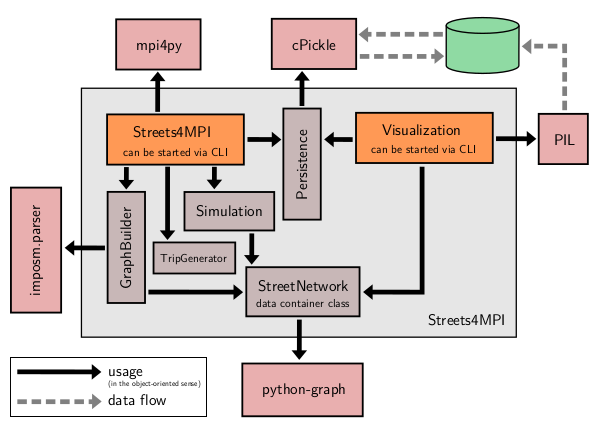
\includegraphics[width=.75\textwidth]{img/architecture_streets4mpi.png}
    \caption{Architecture overview: Streets4MPI~\cite[p. 9]{streets_report}}
    \label{fig:architecture_streets4mpi}
\end{figure}

\textit{streets4MPI} parses \gls{osm} input data, builds a directed graph and repeatedly computes shortest paths for a set amount of ``trips'' (randomly chosen node pairs from the graph) in the graph. Over time it gradually modifies the graph based on results of previous iterations to emulate structural changes in the traffic network in the simulated area. The results can then optionally be written to a custom output format which is visualizable by an additional script~\cite{streets_report}.

As mentioned the applications written in scope of this thesis perform only the graph calculations discarding the produced results. Consequently the implementations do not produce any data besides the runtime statistics externally acquired by benchmark tools.

\section{Differences and limitations}
\label{sec:Concept::Differences}

Although the evaluated implementations are based on the original \textit{streets4MPI}, there are some key implementational differences. This section gives a brief overview over the most important aspects that have been changed and describes both the original application's functionality as well as the derived implementations.

In the remaining part of the thesis the different applications will be referenced quite frequently. For brevity the language implementations to compare will be called by the following scheme: ``streets4<language>''. The Go version for example is called ``streets4go''.

\subsection*{Input format}
\label{subsec:Concept::Differences::Input}

The original \textit{streets4MPI} uses the somewhat dated \gls{osm} \gls{xml} format\fnote{\url{http://wiki.openstreetmap.org/wiki/OSM_XML}} as input which is parsed by \textit{imposm.parser}\fnote{\url{http://imposm.org/docs/imposm.parser/latest/}}. It then builds a directed graph via the \textit{python-graph}\fnote{\url{https://code.google.com/p/python-graph/}} library to base the simulation on~\cite{streets_report}.

The derived versions require the input to be in ``.osm.pbf'' format. This newer version of the \gls{osm} format is based on Google's \gls{protobuf} and is superior to the \gls{xml} variant in both size and speed~\cite{osm_wiki_pbf}. It also simplifies multi language development because the code performing the actual parsing is auto generated from a language independent description file. There are \gls{protobuf} backends for C, Rust and Go which can perform that generation.

\subsection*{Simulation}
\label{subsec:Concept::Differences::Simulation}

The simulation in the base application is based on randomly picked node pairs from the source graph. For these trips the shortest path is calculated by Dijkstra's algorithm as seen in \cite{cormen} and a random factor called ``jam tolerance'' is introduced to avoid oscillation in between iterations~\cite{streets_report}. Then after some time has passed in the simulation, existing streets get expanded or shut down depending on their usage.

The compared implementations of this thesis also perform trip based simulation but without the added randomness and street modification. Also the edge weights are not calculated based on speed limit and length of the street. Instead the derived implementations calculate the length once from the corrdinates of the corresponding nodes and use this as edge weigth directly. The concrete algorithm is a variant of the \shinline{Dijkstra-NoDec} algorithm as seen in~\cite[p. 16]{dijkstra_utcs}. It was mainly chosen because of its reduced complexity in required data structures which again reduces complexity and scope. The algorithm is implemented separately in all three languages so it could theoretically get benchmarked standalone to get clearer results. Mainly because of time constraints this was not attempted in this thesis.

\subsection*{Concurrency}
\label{subsec:Concept::Differences::Concurrency}

\textit{streets4MPI} parallelizes its calculations on multiple processes that communicate via message passing. This is achieved with the aforementioned \textit{MPI4Py} library which delegates to a native \gls{mpi} implementation installed on the system. If no supported implementation is found it falls back to a pure Python solution but the native one should be preferred for maximum performance.

Although Rust as well as Go can integrate decently with existing native code, the reimplementations will be limited to shared memory parallelization on threads. This was mostly decided to evaluate and compare the language inherent concurrency constructs rather than the quality of their foreign funtion interfaces. To achieve a fair comparison \textit{streets4c} will use \textit{OpenMP}~\fnote{\url{http://www.openmp.org}} as it is the de facto standard for simple thread parallelization in C. Of course this solution might not match the performance of hand optimized implementations parallelized with the help of \textit{pthreads} but since the focus is on simple concurrency in the context of scientific applications \textit{OpenMP} was selected as the framework of choice.

\section{Implementation process}
\label{sec:Concept::Implementation}

The implementation process was performed iteratively. Certain milestones were defined and implemented in all three languages. The process only advanced to the next phase when the previous milestone was reached in all applications. This approach was chosen to allow for a fair comparison of the different phases of development. If the implementations would have been developed one after another to completion (or in any other arbitrary order), this might have introduced a certain bias to the evaluation because of possible knowledge about the problem aquired in a previous language translating to faster results in the next one.

\begin{figure}[htb]
    \centering
    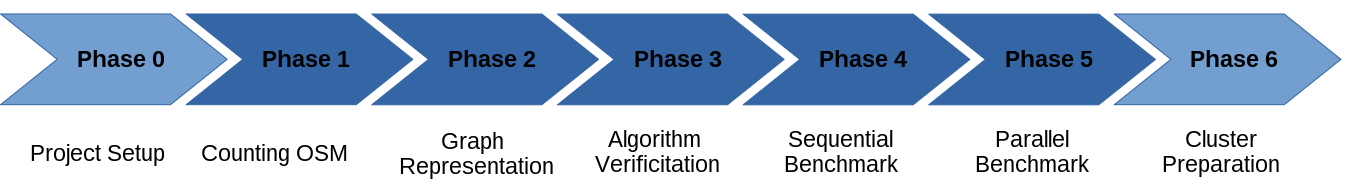
\includegraphics[width=\textwidth]{img/milestone_timeline.png}
    \caption{Milestone overview}
    \label{fig:milestone_timeline}
\end{figure}

\autoref{fig:milestone_timeline} shows the different milestones in order. For each phase various characteristics were captured and compared to highlight the languages' features and performance in the various areas. While the main development and test runs were performed on a laptop the final application was run on a high performance machine provided by the research group Scientific Computing to compare scalability beyond common desktop level processors. In the following sections each milestone is briefly described.

\subsection*{Setting up the Project}
\label{subsec:Concept::Implementation::Setup}

The first phase of development was to create project skeletons and infrastructure for the future development. The milestone was to have a working environment in place where the sample application could be built and executed. While this is certainly not the most important or even interesting part it might show the differences in comfort between the various toolchains.

\subsection*{Counting Nodes, Ways and Relations}
\label{subsec:Concept::Implementation::Counting}

The first real milestone was to read a .osm.pbf file and count all nodes, ways and relations in it. This was done to get familiar with the required libraries and the file format in general. The time recorded began from the initial project created in phase 0 and finished after the milestone was reached. As this is the most input and output intensive phase it should reveal some key differences between the candidates both in speed as well as memory consumption.

\subsection*{Building a basic Graph Representation}
\label{subsec:Concept::Implementation::Graph_Representation}

The next goal was to conceptionally build the graph and related structures the simulation would later operate on. This involved thinking about the relation between edges and nodes as well as the choice of various containers to store the objects efficiently while also keeping access simple. This milestone tested the language's standard libraries and expressiveness in terms of typed containers.

\subsection*{Verifying Structure and Algorithm}
\label{subsec:Concept::Implementation::Verification}

After the base structure to represent graphs and calculate shortest paths was in place it was time to validate the implementations. Unfortunately the OSM data used in the first phase contained too much nodes and ways to be able to efficiently verify any computed results. Therefore a small example graph was manually populated and fed to the algorithm.

\subsection*{Benchmarking Graph Performance}
\label{subsec:Concept::Implementation::SequentialBenchmark}

The fourth milestone was preliminary benchmark of the implementations. The basic idea was to parse the \gls{osm} data used in phase one and build the representing graph. After that the shortest path algorithm is executed once for each node. The total execution time as well as the time taken for each step (building the graph and calculating shortest paths) should be measured and compared as well as the usual memory statistics from previous phases.

\subsection*{Benchmarking Parallel Execution}
\label{subsec:Concept::Implementation::ParallelBenchmark}

The fifth phase consisted of modifying the existing benchmark to operate in parallel via threading and benchmarking the results for various configurations. While all the development and previous benchmarks were performed on a personal laptop the final benchmarks were taken on a computation node of the research group to gather relevant results in high concurrency situations.

\subsection*{Cluster Preperation}
\label{subsec:Concept::Implementation::ClusterPreparation}

The final milestone was to prepare the implementations for the execution on the cluster provided by the research group. As this was a remote environment with some key differences to the development laptop the implementations had to be prepared and slightly changed.

\section{Overview of evaluated Criteria}
\label{sec:Concept::Criteria}

\begin{itemize}
    \item Performance
    \begin{itemize}
        \item Execution Time
        \item Memory Footprint (consumption total + allocation counts)
    \end{itemize}
    \item Productivity
    \begin{itemize}
        \item \acrshort{sloc} Count
        \item Development Time
        \item Tooling Support
        \item Library Ecosystem
        \item Parallelization Effort
    \end{itemize}
\end{itemize}

\section{Related Work}
\label{sec:Concept::Related}

The search for new programming languages which are fit for \gls{hpc} is not a recently developing trend. There have been multiple studies and evaluations but so far none of the proposed languages have gained enough traction to receive widespread adoption. Also most reports focused on the execution performance without really considering additional software metrics or developer productivity~\cite{related_multicore}. at least adds lines of code and development time to the equation but both of these metrics only allow for superficial conclusions about the code quality.

From the candidates presented here Go in particular has been compared to traditional \gls{hpc} languages with mixed results. Although its regular execution speed is somewhat lacking \cite{related_sor_study} showed the highest speedup from parallelization amongst the evaluated languages which is very promising considering high concurrency scenarios like cluster computing. Rust on the other hand has not been seriously evaluated in the \gls{hpc} context probably due to it still being developed.


\chapter{Implementation}
\label{ch:Implementation}

\abstract{This chapter describes the implementation process for all three compared languages. It is divided in sections based on the development milestones defined in the previous chapter~\ref{sec:Approach::Implementation}. The last section briefly describes the preparaton process for the final benchmarks.
}

\setcounter{section}{-1}
\section{Project setup}
\label{sec:Implementation::Setup}

All applications written for this thesis have been developed on Linux thus the setup instructions are for this operating system. They \textit{should} work on *nix as well but there is no guarantee this is the case. Also each section assumes the toolchains for the various languages are installed as this is largely different based on what operating system and on which Linux distribution is used. It is therefore not covered in this thesis.

\subsection{C}
\label{subsec:Implementation::Setup::C}

The buildtool for \textit{streets4C} is GNU \textit{make} with a simple handcrafted \mdinline{Makefile}. It was chosen to strike a balance between full blown build systems like \textit{Autotools}\fnote{\url{http://www.gnu.org/software/software.html}} or \textit{CMake}\fnote{\url{http://www.cmake.org}} and manual compilation. The setup steps required for this configuration are relatively straight forward and listed below.
\\
\lstinputlisting[caption={Project setup: streets4C}, label={lst:setup_c.sh}, style=shell]{code/setup_c}

After creatig a new directory for the application a \mdinline{Makefile} and a sourcefile are created. \mdinline{main.c} contains just a bare bones main method while the \mdinline{Makefile} uses basic rules to compile an executable named \textit{streets4c} with various optimization flags.

All in all the setup in C is quite painless although manual. The only caveat are \mdinline{Makefile}s. They may be simple for small projects without real dependencies but as soon as different source and object files are involved in the compilation process they can get quite confusing. At that point the mentioned build systems might prove their worth in generating the \mdinline{Makefile}(s) from other configuration files.

\subsection{Go}
\label{subsec:Implementation::Setup::Go}

For Go the choice of buildtool is nonexistent. The language provides the \shinline{go} executable which is responsible for nearly the complete development cycle. It can compile your code, install arbitrary Go packages from various sources, run tests and format code just to name the most common features.

This makes Go (the language) extremely convenient since everything you want to do is probably one commandline away. For example to get a dependency one would invoke the tool like so: \mdinline{go get github.com/petar/GoLLRB/llrb}. This will download the package in source form which can then be imported in any project on that machine via its fully qualified package name.

To achieve this convenience the \shinline{go} tool requires some setup work before it can be used for the first time. Because of this this section contains two setup examples.
\\
\lstinputlisting[caption={Project setup: streets4Go}, label={lst:setup_go.sh}, style=shell]{code/setup_go}

Listing \ref{lst:setup_go.sh} describes the steps that were taken to create the \textit{streets4Go} project inside the thesis's repository. It is pretty similiar to the C version. A directory gets created then a source file containing a \shinline{main} function is created which can be built and run with a single command. Unfortunately this variant does not follow the guidelines for project layout as described in \href{https://golang.org/doc/code.html#Workspaces}{the official documentation} because the code does not live inside the globally unique \shinline{GOPATH} folder.

To be able to download packages only once the \shinline{go} commandline utility assumes an environment variable called \shinline{GOPATH} is configured to point to a directory which it has full control over. This directory contains all source files as well a the compiled binaries all stored through a consistent naming scheme. Normally it is assumed that all Go projects live inside their own subdirectories of the \shinline{GOPATH} but it is possible to avoid this at the cost of some convenience.

The project that was created through the commands of \autoref{lst:setup_go.sh} for example cannot be installed to the system by running \mdinline{go install} since it does not reside in the correct folder instead one has to copy the compiled binary to a directory in \shinline{PATH} manually.

The next \hyperref[lst:setup_go_full.sh]{Listing} shows a more realistic workflow for creating a new Go project from scratch without any prior setup required. It expects the programmer to start in the directory that should be set as \shinline{GOPATH} and uses \href{https://www.github.com}{\shinline{GitHub}} as code host which in reality just determines the package name. It is also important to add the export shown in the first line to any inititalization file of your shell or operating system to ensure it is accessible everywhere.
\\
\lstinputlisting[caption={Full setup for new Go projects}, label={lst:setup_go_full.sh}, style=shell]{code/setup_go_full}

\subsection{Rust}
\label{subsec:Implementation::Setup::Rust}

Similar to Go also Rust provides its own build system. As mentioned in the \hyperref[subsec:State_of_the_art::Candidates::Rust]{candidate introduction} Rust installs its own package manager \textit{cargo}. It functions as build system and is also capable of creating new projects. This shortens the setup process considerably as observable in the next \hyperref[lst:setup_rust.sh]{Listing}.
\\
\lstinputlisting[caption={Project setup: streets4Rust}, label={lst:setup_rust.sh}, style=shell]{code/setup_rust}

With the \shinline{new} subcommand a new project gets created. The \shinline{-{}-bin} flag tells \shinline{cargo} to create an executable project instead of a library which is the default.
Thanks to the one command all the initial files and directories are created with one single command. This includes:
\begin{itemize}
    \item{the project directory itself (named like the given project name)}
    \item{a \mdinline{src} directory for source files}
    \item{a \mdinline{target} directory for build results}
    \item{a required manifest file named \mdinline{Cargo.toml} including the given project name}
    \item{a sample file inside \mdinline{src} which is either called \mdinline{main.rs} for binaries or \mdinline{lib.rs} for libraries containing some sample code
    \item{and optionally an empty initialized version control repository (\shinline{git} or \shinline{mercurial} if the corresponding command line option has been passed)}
\end{itemize}
The resulting application is already runnable via \shinline{cargo run}\footnote{Which is executable anywhere inside the project directory} and produces some output in \shinline{stdout}. This process is extremely convenient and error proof since \shinline{cargo} validates all input before executing any task. The \shinline{man} pages and help texts are quite thin at the moment but as with everything in the Rust world \shinline{cargo} is still in active development.

The overall greatest advantage however is that the Rust process does not involve any manual text editing. What might sound trivial at first, is actually quite important for newcomers to the language. You do not have to know any syntax to get started with Rust since the generated code already compiles and does something interesting. In the other languages you have to write a valid, minimal program manually to even test the project setup while Rust is ready to go after just one command.

Of course this strategy is not without limitations. To be able to use \shinline{cargo} all files and directories have to follow a special pattern. Although the chosen conventions are somewhat common one cannot use arbitrary directory and file names.

\subsection{Comparison}
\label{subsec:Implementation::Setup::Comparison}

For newcomers Rust definitely provides the best experience. One can get a valid \textit{Hello world!} application up and running without any prior knowledge which lowers the barrier of entry dramatically. In addition Rust does not require any presetup before the first project. Just install the language toolchain (either through the operating system's package manager or the very simple setup script\fnote{\url{https://static.rust-lang.org/rustup.sh}}) and start coding.

Go requires some intial setup besides the installation but is still quite easy to setup. The \shinline{GOPATH} exporting is a small annoyance but it balances out with the benefits the developer gets later down the line like easy dependency management. The syntax is very concise so creating a new source file with a \shinline{main} function is still quite fast.

Considering C's long lifespan the tooling for project setup is not very good. Full blown IDEs like Eclipse provide wizards to create all required files but for free standing development with a simple text editor and GNU \textit{make} there is no real automation possible. Naturally it is not hard to create an empty C source file however the compiler and linker usability is still years behind other modern toolchains. One example is linking libraries where the developer can decide between potentially unneeded libraries being included in the application (with default settings) or having to carefully order the linker arguments (with the special flag \shinline{-{}-as-{}-needed}) which is tedious when new dependencies get added later on.

This probably does not apply to seasoned C developers and one could make the argument that it is inherent to the language's ``closeness to the metal''. But acknowledging the fact that scientists of other fields more often than not see programming as an unwanted necessity to be able to complete their research it is questionable whether this technical know-how should really be required to use a language like C.

\section{Counting nodes, ways and relations in an .osm.pbf file}
\label{sec:Implementation::Counting}

\begin{table}[htb]
    \centering
    \begin{tabular}{llll}
        \toprule
        % Header
            & C
            & Go
            & Rust \\
        \midrule

        \gls{sloc}
            & 163
            & 55
            & 36 \\

        Development time (hours)
            & 00:51:18
            & 00:21:16
            & 00:33:09 \\

        Execution time (sec)
            & 1.017 (-O0)
            & 4.846 (GOMAXPROCS=1)
            & 27.749 (-O0) \\
            & 0.994 (-O3)
            & 1.381 (GOMAXPROCS=8)
            & \hspace{6pt}2,722 (-O3) \\

        Allocation count
            & 2,390,566
            & 11,164,068\fnote{The memory statistics for Go have not been acquired by \textit{valgrind} but by \shinline{runtime.MemStats}}\textsuperscript{,}\fnote{The fact that Go is garbage collected explains the discrepancy in allocations and frees}
            & 11,373,558 \\

        Free count
            & 2,390,566
            & 11,000,199
            & 11,373,557\fnote{This is due to a bug in the osmpbf library used. In safe Rust code it is very hard to leak memory (usually involving reference cycles or something similar).} \\
        \bottomrule
    \end{tabular}
    \caption{Milestone 1: Counting nodes, ways and relations}
    \label{tb:milestone1}
\end{table}

\subsection{C}
\label{subsec:Implementation::Counting::C}

Preface: For the first real milestone \textit{streets4C} had an important disadvantage. There was no library to conveniently process \gls{osm} data. Therefore a small abstraction over the offical \gls{protobuf} definitions had to be written. The development time for this code located in \mdinline{osmpbfreader.c/h} was not counted towards the total time of the phase to avoid unfair bias just because of a missing library however the \gls{sloc} count includes the additional code since it was essential to this stage.

The first phase of development already highlighted many of the common problems encountered when programming in the C language. After finishing the aforementioned library it had to be included in the development process which in return meant the \mdinline{Makefile} had to be extended to also compile \mdinline{osmpbfreader.c} and include the resulting object file in assembling the executable binary. This proved harder than expected which can partly be attributed to the author's lacking expertise with the C compilation process but also confirms the unneeded complexity of such a simple task.

Ultimately the problem was the order in which the source files and libraries were passed to the compiler and linker. The libraries were included too early which resulted in ``undefined reference to method'' error messages because the aforementioned linker flag \shinline{-{}-as-{}-needed} was enabled per default by the Linux distribution. In this mode the linker effectively treats passed objects files as completed when no missing symbols are found after the unit has been processed and therefore ignores them in the further linking process. As a result the arguments have to carefully match the dependency hierarchy to not accidentally remove a critical library early on so that later files cannot use their symbols.

In times where compilers are smart enough to basically rewrite and change code for performance reasons it is completely inexcusable that the order of source arguments to process is still that relevant. Meanwhile other toolchains show that it is definitely possible to accept arguments in arbitrary order and perform the required analysis whether to include a given library in a second pass. This effectively combines the best of both inferior strategies the C linker currently supports. The time spent solving these compilation errors shows in the statistics for C which is considerably larger than its competitors in this stage.

The other big caveat in working with \gls{osm} data was the manual memory management. Since said data is stored in effectively compressed manner in the file additional heap allocations were unavoidable in accessing it. This requires either explicit freeing by the caller or a symmetric deallocation function provided by the library. In the case of \gls{protobuf} it is even worse since a client cannot just perform the usual \shinline{free()} call but has to use the custom freeing functions generated from the source \shinline{.proto} format description files. For some intermediate allocations it is possible to limit this to the body of a libaray function but on the real data it shifts additional responsibilities on the caller.
\\
\lstinputlisting[caption={Manual memory management with Protobuf in C}, label={lst:manual_pbf_freeing.c}, style=c]{code/manual_pbf_freeing.c}

\autoref{lst:manual_pbf_freeing.c} shows this overhead introduced by the mandatory call to \shinline{osmpbf\_\_primitive\_block\_\_free\_unpacked} in line 17. This results in some very asymmetric interface design since the parsing library has to rely on the client application to explicitly call the correct free function from the \gls{protobuf} library. While this approach is acceptable for regular allocations via the C standard library, it is a problem here since the allocating function's name \shinline{get\_next\_primitive} does not directly imply a heap allocation (and the resulting need to free it later).

Considering this fact the \gls{sloc} count is still decent. With the help of a clever library interface the overhead for the memory management is comparatively small and the data is even loopable by a \shinline{while} loop which allows for convenient access and conversion. Also the statistics clearly show why C is still that dominant in the \gls{hpc} area. With low allocation counts\fnote{Although these are also partially caused by the simplicity of the custom osmpbfreader abstraction} and superior singlethreaded(!) performance C is the clear winner in the performance area for this first milestone.

\subsection{Go}
\label{subsec:Implementation::Counting::Go}

To parse the .osm.pbf files \textit{streets4Go} uses an existing library simply called \textit{osmpbf}\fnote{\url{https://github.com/qedus/osmpbf}}. The library follows common Go ``best practices'' which makes it easy to use. Internally goroutines are used to decode data in parallel which can then be retrieved through a \shinline{Decoder} struct. The naming of the struct and the corresponding methods follow the conventions of the official Decoder types of the Go standard library. This adherence to conventions directly shows in the development time which is the shortest amongst the candidates for this first phase.
\lstinputlisting[caption={Dependency management in Go}, label={lst:dependency_management.go}, style=go]{code/dependency_management.go}

Dependency management was very easy and intuitive. As mentioned in the \hyperref[subsec:State_of_the_art::Candidates::Go]{candidate introduction} \mdinline{go get} was used to download the library and a simple import statement was enough to pull in the necessary code (see \autoref{lst:dependency_management.go}). One caveat here are once again Go's strict compilation rules. Since an unused import is a compiler error an editor plugin kept deleting the prematurely inserted import statement as part of the saving process. While the auto fix style of tools like \shinline{gofmt} and \shinline{goimports} is certainly helpful for fixing common formatting errors, the loss of control for the developer takes some time to get used to.

Another interesting recorded statistic is the count of \acrlong{sloc}. This count exposes one of the criticisms commonly directed at Go - verbose error handling. Although the code is semantically simpler (no manual memory management, higher level language constructs) the \gls{sloc} count is in fact identical to that of \textit{streets4C}. This is partially the result of the common four line idiom to handle errors. A function that could fail typically returns two values. The desired result and an error value. If the function failed to execute successfully the error value will indicate the source of the failed execution. Otherwise this value will be \shinline{nil} signalling a successful completion. This pattern is used three times in this simple first phase alone which results in 12 lines.
\\
\lstinputlisting[caption={Idiomatic error handling in Go}, label={lst:error_handling.go}, style=go]{code/error_handling.go}

Considering the aforementioned simplicity \textit{streets4Go}'s performance characteristics are very promising. Although in its basic form about four to five times slower than the C solution the parallelized version achieves similar performance to \textit{streets4C}. This version was only included since the library was already based on a variable number of \glspl{goroutine} which made the parallelzation a matter of changing an environment variable in the Go runtime. While this change required only the addition of a single line, the C abstraction \shinline{osmpbfreader} might not even be parallelizable without considerable changes to its architecture. This truly shows the power of language level parallelization mechanics and confirms the choice of Go as a candidate in this evaluation.

\subsection{Rust}
\label{subsec:Implementation::Counting::Rust}

\textit{streets4Rust} also had the advantage of an existing library to use for \gls{osm} decoding which is called \textit{osmpbfreader-rs}\fnote{\url{https://github.com/texitoi/osmpbfreader-rs}}. Similar to Go the dependency management was extremely convenient and simple. The only changes necessary were an added line in the Cargo manifest (\mdinline{Cargo.toml}) and an \shinline{extern crate osmpbfreader;} in the crate root \mdinline{main.rs}. After that \mdinline{cargo build} downloaded the dependency (which in this case meant cloning the \shinline{Git} repository) and integrated it into the compilation process.

Compared to C and Go \textit{streets4Rust} required a medium amount of development time and had the lowest \gls{sloc} count in this phase. This can mainly be attributed to the library's use of common Rust idioms and structures like \shinline{iterators} and \shinline{enumerations}. Unlike their C equivalent, which are basically named integer constants, Rust enumerations are real types. This means they can be used in pattern matching expression and act as a target for method implementations similar to structures. The next \hyperref[lst:osm_decoding.rs]{Listing} shows the complete decoding part of this stage which is very compact and easy to understand thanks to Rust's high level constructs.
\\
\lstinputlisting[caption={\gls{osm} decoding in Rust}, label={lst:osm_decoding.rs}, style=rust]{code/osm_decoding.rs}

The function \shinline{blocks::iter} returns an enum value which gets pattern matched on to determine which counter should get incremented. While this example does not actually use any fields of the objects it would be a simple change to destructure the enum values and retrieve the structures containing the data rom within.

The execution time highlights another important factor in regards to Rust's matureness as a language. The optimized version is more than ten times faster then the binary produced by default options. This is mostly due to the fact that the Rust \gls{llvm} frontend produces bloated byte code which does not get optimized on regular builds. That is also the reason release builds take substanstially longer. It simply takes more time to optimize (and therefore often shrink) \gls{llvm_ir} instead of emitting less code in the first place. Although the code generation gets improved steadily it is not a big focus until version \shinline{1.0} is released but the Rust core team knows about the issue and it is a high priority after said release.

Nonetheless the release build shows the power of \gls{llvm}'s various optimization passes. \textit{streets4Rust} achieves the second best single threaded performance after C with a run time of 2.72 seconds which is impressive considering the vastly shorter development time and lowest \gls{sloc} count across all candidates.

\subsection{Comparison}
\label{subsec:Implementation::Counting::Comparison}

\section{Building a basic graph representation}
\label{sec:Implementation::Graph_Representation}

The second milestone was to develop a graph structure to represent the street network in memory. Like in \textit{streets4MPI} random nodes from this data would then be fed to Dijkstra's shortest path algorithm to simulate trips. Since all applications should be parallelized later on the immutable data (such as the edge lengths, \gls{osm} ids and adjacency lists) needed to be stored separately from the changing data the algorithm required (such as distance and parent arrays). To achieve this all implementations provide a \shinline{graph} structure holding the immutable data and a \shinline{dijkstragraph} structure to store volatile data for the algorithm alongside some kind of reference (or pointer) to a graph object.

Since this milestone included a preliminary implementation of the actual algorithm it required the use of a priority queue which was not directly available in all languages. Considering this fact the third milestone already highlighted some differences in comprehensiveness of the different standard libraries.

\begin{table}[htb]
    \centering
    \begin{tabular}{llll}
        \toprule
        % Header
            & C
            & Go
            & Rust \\
        \midrule

        \gls{sloc} (total)
            & 385
            & 196
            & 170 \\

        Development time (hours)
            & 02:30:32
            & 01:06:06
            & 01:14:28 \\
        \bottomrule
    \end{tabular}
    \caption{Milestone 2: Building a basic graph representation}
    \label{tb:milestone2}
\end{table}

\subsection{C}
\label{subsec:Implementation::Graph_Representation::C}

As seen in \autoref{tb:milestone2} this stage resulted in a much higher \gls{sloc} count for C. This is due to the fact that development took place in another source files. To encapsulate graph functionality properly a new file called \mdinline{graph.c} was created. Following established conventions this meant also creating a matching header (\mdinline{graph.h}) to be able to use the newly written code in the main application. While this separation is decently useful to not have to clobber you source file with structure definitions it also introduces a fair bit of redundancy. Functions are declared in the header and implemented in the source files which means the signature appears twice. In addition C had the unfortunate problem of not having a proper implementation of a priority queue easily available which required the addition of another source file / header combination (\mdinline{util.c/h}). This increased the \gls{sloc} count even further and added some additional development time as well.

At this point it became clear the C version would not be created dependency free. Advanced data structures such as hash tables or growing arrays are essential when properly modelling a graph and the choice was made to use the popular \textit{GLib}\fnote{\url{https://developer.gnome.org/glib/stable/}} to provide these types. It is a commonly used library containing data structures, threading routines, conversion functions or macros and much more. Since both Rust and Go's standard library are much more comprehensive then C's the addition of GLib to the project is easily justified.

Implementing the graph representation itself was very straight forward. Similar to the mathematical representation a \shinline{graph} in \textit{streets4C} consists of an array of \shinline{node}s and \shinline{edge}s. To be able to map from \gls{osm} ids to array indices two hash tables were added using \lstinline[style=c]{long}s as keys and \lstinline[style=c]{int}s as values. The \shinline{dgraph} structure can be created with a pointer to an existing \shinline{graph} and is then able to execute Dijkstra's \acrshort{sssp} algorithm.
\\
\lstinputlisting[caption={Graph representation in C}, label={lst:graph_representation.c}, style=c]{code/graph_representation.c}

All structures contain little more than the expected data besides the \shinline{cur} field in \shinline{dgraph}. It had to be added since Glib's \shinline{GHashTable} only supports operations on all key-value-pairs via a function pointer with a single extra argument. Since the algorithm requires access to the currently explored node's index as well as the distance and parent arrays the index needs to be stored in the struct itself.

While the extra field was a minor inconvenience other problematic aspects were the code bloat and additional unsafety introduced by the use of \shinline{GHashTable}s\fnote{The hash table implementation provided by GLib}. Since C is not typesafe by design and also does not allow for true generic programming via type parameters nearly all generic code is written using \lstinline[style=c]{void*}. This leads to very verbose code because of the high amount of casts involved when accessing or storing values inside a \shinline{GHashTable} or \shinline{GArray}.

Another complication was the use of integers as keys in \shinline{GHashTable}. It requires both key and value to be a gpointer (which is a platform independent \lstinline{void} pointer) which forces the programmer to either allocate the integer key on the heap or explicitly cast it to the correct type. This works well using a macro provided by GLib until the number zero appears as a value because it represent the \shinline{NULL} pointer which GHashTable also uses to indicate a key was not found in the hash table. Although there is an extended function which is able to indicate to caller whether the return value is \shinline{NULL} because it was stored that way or because it was not found, this problem could have been avoided by a better \acrshort{api} design.

The implementation of Dijkstra's algorithm was not particularly hard only more verbose than expected. As mentioned the GHashTable only provides iterative access through an extra function. As a consequence the step commonly referred to as \textit{relax edge} is contained in a separate function that get passed to \shinline{g\_hash\_table\_foreach}. In combination with the conversion macros and temporary variables the code bloats up.

All in all the experience was poor compared to the other languages. The verboseness and missing safety lead to the highest development time and \gls{sloc} count by far. The time was spent debugging some obscure errors introduced by the excessive casting which might have been avoided by a more sophisticated typesystem.

\subsection{Go}
\label{subsec:Implementation::Graph_Representation::Go}

In Go the graph is again mostly composed of two arrays holding all nodes and edges. However Go's \shinline{slices} and \shinline{maps} are dynamically growing. This means the constructor function of the graph does not require capacity parameters to intialize these fields since they can reallocate if neccessary. In general the development process was once again very smooth and simple which shows in the short time spent and the low \gls{sloc} count.
\\
\lstinputlisting[caption={Graph representation in Go}, label={lst:graph_representation.go}, style=go]{code/graph_representation.go}

\hyperref[lst:graph_representation.go]{Listing} shows that the structures are nearly identical to their C counterparts. Only the current node index in DijkstraGraph was not required since Go allows for much better iteration through maps. It is also interesting to note that Go supports (and even encourages) the declaration of multiple fields of the same type on the same line. Although this was used only two times in the snippet it shrinks the line count while keeping the code understandable since two fields with identical types are often related anyway.

As stated in the \hyperref[sec:Implementation::Graph_Representation]{introductory part} Dijkstra's algorithm depedends on a priority queue. Despite the fact that Go's standard library does not directly provide a ready-to-use implementation thereof the required steps to achieve this were minimal. The package \shinline{container\textbackslash heap}\fnote{\url{http://golang.org/pkg/container/heap/}} offers a convenient way to work with any kind of heap. The only restriction is that the underlying data structure implements a special interface containing common operations used to \textit{heapify} the stored data. Since interfaces are implicitly implemented on all structures which present the necessary methods it was a simple task to create a full featured priority queue on top of a slice by writing just four trivial methods.
\\
\lstinputlisting[caption={Priority queue in Go}, label={lst:priority_queue.go}, style=go]{code/priority_queue.go}

While the heap implementation was provided by the standard library (which is likely to be correct) it required the custom methods of \autoref{lst:priority_queue.go} to be correct. At this point Go's builtin test functionality came in handy. All it took to test the custom implementation was to create another file called \shinline{util\_test.go} (the suffix ``\_test.go'' is mandatory) and write a simple test. No import besides the \textit{testing} package were needed since the code resided in the same package as the main application and all tests got executed with a single call of \mdinline{go test}. In contrast the C implementation required the setup of an additional source file including a regular main function which then had to be manually compiled and run. In addition some basic error formatting and output had to be written to properly locate potential errors in the implementation. Although all test related statistics are not counted in either language, Go's testing workflow is clearly superior to the manual, errorprone C approach.

All things considered this milestone was easily implemented in Go. The builtin container datastructures simplified the structure definitions while the provided heap implementation had a very low entry barrier and produced quick results. This is reflected in the statistics which are on par with the Rust version discussed in the next section.

\subsection{Rust}
\label{subsec:Implementation::Graph_Representation::Rust}

The original plan for the Rust implementation was to use direct references between nodes and edges of the graph to allow for easy navigation during the algorithm. Combined with the guarantees the typesystem offers it seemed to be a unique approach offering both convenient access and memory safety. Unfortunately this approach was quickly dismissed since it would have essentially created circular datastructures. While those are definitely possible to implement, it takes some \shinline{unsafe} marked code and a lot of careful interface design to retain the aforementioned safety. Due to, once again, time restrictions an architecture similar to the Go and C variant was implemented.

The interesting differences in contrast to the previously introduced structures are located in \shinline{DijkstraGraph}. The \shinline{queue} field has the type \shinline{BinaryHeap} which is located in the standard library. This already shows that Rust is the only language out of the candidates which contains a complete implementation of this datastructure as part of the core libraries. While a priority queue is certainly not an essential component of every program it was required for this algorithm and having it available right from the start was beneficial to the development.
\\
\lstinputlisting[caption={DijkstraGraph in Rust}, label={lst:graph_representation.rs}, firstline=24, style=rust]{code/graph_representation.rs}

The other interesting part is the type of the \shinline{graph} field. As mentioned earlier the struct calculating the shortest paths needs a reference to the immutable graph data. Ideally one would like to encode this immutability in the type itself. This is where Rust's typesystem shines. As mentioned in the \hyperref[subsec:State_of_the_art::Candidates::Rust]{language introduction} regular references only allow read access. This means DijkstraGraph cannot (accidentally or intentionally) modify the referenced Graph instance or any of its fields just because the reference does not allow this. This comes in handy later in a parallel scenario where multiple threads are reading data from the graph while calculating shortest paths. The readonly reference (in Rust terms ``a shared borrow'') ensures no data races can happen when accessing the graph concurrently.

From a statistics standpoint Rust is evenly matched with Go. While \textit{streets4Go} took a little less time to write, \textit{streets4Rust} has a few less lines. This mostly came down to the heap implementations being available in the standard library (which means less code had to be written) and the mentioned deviation from the original implementation plan, adding some additional development time.

\subsection{Comparison}
\label{subsec:Implementation::Graph_Representation::Comparison}

Although this milestone did not contain any performance measurements it clearly highlighted and emphasized the original argument for a new language in \acrlong{hpc}. In scenarios where complex data structures beyond a simple array are required C fails to deliver an easy development experience. This was mostly due to the lack of ``true'' generic programming limiting the expressiveness of the implemented structures and algorithms. Since all casts in C are unsafe anyway but required to enable genericity, one slight type error, which a rigid typesystem might have prevented from even compiling, can cause segmentation faults which are hard to trace and correct. This clearly underlines that C is not the optimal choice for developing complex high performance applications.

Go and Rust performed equally well in this stage. Both include a typesystem suited to safely use generic containers and provide a sufficient standard library for a decent implementation of a shortest path algorithm. Although Go's generics are limited to builtin types like slices and maps this was not an issue in this stage since no generic methods had to be written. Rust had the unique advantage to be able to express application semantics (graph data is immutable to the algorithm) in the typesystem. Although that did not solve any immediate problems in the implementation it can help to prevent a whole class of defects as described in the previous section.

\section{Verifying structure and algorithm}
\label{sec:Implementation::Verification}

The next goal was to verify the implemented algorithms on some sample data. To achieve this a sample graph with ten nodes and about 15 edges was constructed followed by a shortest path calculation for each node. Although performance was measured it was not the core focus of this stage since the input data was very small and not representative of the \gls{osm} data. Nonetheless the execution time reveals some interesting differences between the competitors.

\begin{table}[htb]
    \centering
    \begin{tabular}{llll}
        \toprule
        % Header
            & C
            & Go
            & Rust \\
        \midrule

        \gls{sloc} (total)
            & 633
            & 275
            & 232 \\

        Development time (hours)
            & 01:53:30
            & 01:16:49
            & 01:04:38 \\

        Execution time (seconds)
            & 0.004 (-O0)
            & 0.686
            & 0.007 (-O0) \\
            & 0.003 (-O3)
            & % intentionally blank since no parallel version was build
            & 0.005 (-O3) \\

        Allocation count
            & 108
            & 519
            &  47 \\

        Free count
            & 106\fnote{Due to the use of GLib some global state remains reachable after exiting. This is likely intended behaviour and not a memory leak (see: \url{http://stackoverflow.com/a/4256967}).}
            & 169
            &  47 \\

        Allocation amount (bytes)
            & 7,868\fnote{2,036 bytes were in use at exit see footnote 14}
            & 53,016
            & 22,792
        \bottomrule
    \end{tabular}
    \caption{Milestone 3: Verifying the implementation}
    \label{tb:milestone3}
\end{table}

\subsection{C}
\label{subsec:Implementation::Verification::C}

Unsurprisingly the C implementation has the lowest execution time among the compared languages. Unfortunately the performance was once again paid with a high development time following the trend from previous milestones. In this phase a lot of time was invested into debugging the custom priority queue implementation. Although there was a simple test performed in the last stage the real data revealed a bug when queuing zero indices. Similar to the GHashTable the zero index was casted to a void pointer and treated as null which caused errors during the pop operation later on. Unfortunately the defect manifested in the typical C style with a nondescriptive segmentation fault.

Performancewise C proves once again why it is one of the two major players in \gls{hpc}. The execution time is unbeaten (even unoptimized) and the allocation amount is the lowest among the contestants by far. As explained in the annotation the mismatch in \shinline{malloc} and \shinline{free} calls can be explained by the inclusion of GLib. For its advanced features like memory pooling it retains some global state which \textit{valgrind} mistakenly classifies as a potentital leak.

\subsection{Go}
\label{subsec:Implementation::Verification::Go}

The verification in Go took a little bit longer than expected. Although the implementation itself was quickly completed it exposed some errors in the original graph structure. The main problem was the initialization of the graph slices. The previous implementation used the builtin function \shinline{make} to create a slice with an initial capacity. When adding nodes to the slice later another builtin function \shinline{append} was used under the assumption the slice would be empty initially. This was not the case since Go had just filled the whole slice with empty node objects. This caused errors later down the line when these empty objects were used in Dijkstra's algorithm. The problem was later solved by changing the creation function from \shinline{make} to \shinline{new}. This method just creates a new array and lets the slice point into it reallocating later if neccessary.

While the actual change in code was minimal the origin of this defect is interesting. As mentioned above all three functions interacting with the slice are built into the language itself. This approach was explicitly chosen to make common operations (like creating, retrieving the length or capacity) on common types (like slices, arrays and maps) more accessible. Unfortunately these functions obviously have slightly different meanings on different types resulting in some unexpected behaviour. This is certainly something which can be picked up when using Go for extended periods of time but especially for newcomers it can cause some confusion and while the new variant with \shinline{new} works it is unclear whether this is the ideomatic way to create growing slices.

From a performance standpoint \textit{streets4go} falls short compared to the other implementations. This can mostly be explained by the Go runtime. It needs some initial setup time and memory which increases the allocation amount and prolongs execution time. Since this was a very small benchmark only used to validate the implementations these little ``static costs'' make up a much higher percentage of the total statistics.

\subsection{Rust}
\label{subsec:Implementation::Verification::Rust}

During the implementation an effort was made to randomize the order of languages between milestones. It just happened that Rust was the last candidate in this phase since an update in the nightly version of the compiler broke the \gls{protobuf} package on which the \gls{osm} library depended on. Although the author was quick to update the code to the changes there was a downtime of about three to four days where the development could not continue since the other versions were finished but \textit{streets4Rust} did not build. Although this was the only case where the code was majorly broken for larger timespan it still effectively halted the whole process. Luckily the first stable release is scheduled for shortly after the deadline of this thesis so this should not really be a problem later on.

In this case it was even an advantage that the Rust version was developed last since it revealed a critical error in the other implementations. When creating the sample graph all data was derived from indices of two for loops. The assumption was that edges created in the second loop would only reference existing nodes created in the first one. Since both other implementations did not crash or produce any errors the creation code was not thoroughly verified. Running the same sample data through the Rust application revealed the error. The \shinline{add\_edge} method did not check whether the edge ids passed as arguments were previously added to the graph. This is mandatory since the ids get converted to array indices to be able to add the nodes in the respecting adjacency lists. A map lookup in Go or C is achieved via the indexing operator which then returns and the value element associated with the given key. Obviously this operation can fail when the given key is not found in the map. While both C and Go indicate this error case with a return of zero the possibility of failure is directly encoded in the corresponding Rust. Instead of simply returning the value it returns an \shinline{Option} which is a Rust enumeration is either containing a value or \shinline{None}. This type is a perfect fit for functions which might fail to return the desired value since it shifts the responsibility to deal with the failure to the callee which can potentially recover or otherwise abort completely. The following Listings show the id to index conversion in Go and Rust highlighting the differences.
\\
\lstinputlisting[caption={Map lookup in Go}, label={lst:map_lookup.go}, style=go]{code/map_lookup.go}
\\
\lstinputlisting[caption={Map lookup in Rust}, label={lst:map_lookup.rs}, style=rust]{code/map_lookup.rs}

Although not shown here the C version behaves identical to the Go version but uses a static function \shinline{g\_hash\_table\_lookup}. While the indexing seems more convenient is does not offer precise feedback over the success state of the operation. In this context this is especially critical since zero is a semantically valid index to retrieve. As mentioned above the return value of Rust's \shinline{HashMap.get} is an \shinline{Option} and as such it has to be ``unwrapped'' to get the contained value. This method panics the thread if called on a \shinline{None} value which is exactly what happened when the application processed the sample data. Further investigation then revealed a missing check whether the key is contained in the map which got silently ignored in both other applications. This is a good exaple of how a sophisticated typesystem can prevent potential errors through descriptive types.

The statistics for this milestone are once again very promising for Rust. With the lowest \gls{sloc} count as well as develoment time it still remains competitive with the execution performance of C. The allocation count also hints that Rust's vectors probably have a bigger reallocation factor than the GHashTable from GLib. While the count of function calls is smaller the amount of memory allocated is larger.

\subsection{Comparison}
\label{subsec:Implementation::Verification::Comparison}

This milestone highlighted the importance of strong typesystems in particular. They can prevent bugs which would otherwise require intensive testing to be even noticed in the first place. Rust shines in this discipline. Its typesystem not only pretty much guarantees memory safety but also allows libraries to encode usage semantics into function signatures preventing some cases of possible misuse. In addition C once again comes in last in terms of developer productivity and while the performance benefit is still in its favor Rust reaches a similar speed which took only about half as long to implement. While Go is certainly not as fast as the other two languages as of yet it is a very comfortable language and allows for some decent productivity gains.

\section{Sequential benchmark}
\label{sec:Implementation::SequentialBenchmark}

In this milestone runtime performance came back into the main focus. Since the algorithms at this point were proven to work correctly it could now be applied to real geographical data. The main technical challenge here was to efficiently process the input file while ideally directly filling the graph with the accumulated data. The caveat was the handling of \gls{osm} \shinline{ways} which are later represented by one or more edges in the graph. The input format lists all ids of the nodes which are part of the way but these nodes might not have been processed and added to the graph yet. This forced the implementations to retain the ways' data in some way and construct edges from that data in a second step.

\begin{table}[htb]
    \centering
    \begin{tabular}{llll}
        \toprule
        % Header
            & C
            & Go
            & Rust \\
        \midrule

        \gls{sloc} (total)
            & 757
            & 359
            & 292 \\

        Development time (hours)
            & 01:14:32
            & 00:56:16
            & 00:45:20 \\

        Execution time (hours)
            & 08:34:01 (-O3)
            & 09:08:19
            & 07:31:37 (-O3) \\

        Memory usage (MB)\fnote{Obtained via htop (\url{http://hisham.hm/htop/}) at the time of shortest path calculation}
            & 994
            & 1551
            & 2235 \\

        \bottomrule
    \end{tabular}
    \caption{Milestone 4: Sequential benchmark}
    \label{tb:milestone4}
\end{table}

\subsection{C}
\label{subsec:Implementation::SequentialBenchmark::C}

For \textit{streets4C} the most time was spent on dealing with the edges. As mentioned in the introductory part they need to be saved and added later. This either required knowing the amount of edges beforehand (to be able to preallocate an array large enough to store all information) or to use a dynamically growing array to store them as they get processed. Since the amount of edges is not stored in the \gls{osm} file, the first approach would have to read the whole input file twice to count edges (and ideally nodes too) first and then parse the actual data in the second run. To prevent this the second design was chosen and implemented.

Of course self-reallocating arrays are not part of the C language or standard library and so the application had to rely on GLib once again. The used types were \shinline{GPtrArray} to store pointers to the heap allocated \textit{node} and \textit{edge} structures and the regular \shinline{GArray} to store the \gls{osm} ids of the constructed edges. With this implementation the file only needed to get read once creating the actual values and counts (useful to pass to the graph creation method as capacities later) in the process.

Another option would have been to rewrite part of the graph structure to use GArrays internally for storing edges and nodes in the first place. This idea was not realized to keep the number of external data structures in the graph representation minimal. However that change would have simplified this milestone considerably.

The performance statistics from this phase contain the first real surprise. \textit{streets4C} does not have the lowest execution time and Rust outshines the C implementation by more than an hour. This might reflect a suboptimal architecture on the C side which can be traced back to the author's limited experience with the language. However this might very well be reflective of a scientist with similarly limited programming skills. Considering the development time and \gls{sloc} count the result is even more alarming. The redeeming factor for C is the memory footprint which is the lowest among the three languages. Although memory is typically not as critical as processing time it is still an important criteria when evaluating \gls{hpc} applications and has to be taken into account.

\subsection{Go}
\label{subsec:Implementation::SequentialBenchmark::Go}

This phase did not offer any difficult technical challenges for the Go implementation. Nodes could be added right as they were encountered while parsing whereas edges were temporarly stored in a growing slice and were appended in a second pass.

An essential function for this milestone was the calculation of the length between two nodes based on latitude and longitude. Based on \textit{streets4MPI} the haversine formula\fnote{\url{http://en.wikipedia.org/wiki/Haversine_formula}} was chosen to perform this calculation. This kind of mathematical formulae can be implemented very compactly in Go. Especially the assignments of multiple variables in the same line helps readability and reduces the amount of lines required.

While the \hyperref[lst:haversine.go]{following Listing} is a bit small in width the advantages should be clearly visible. The multiline assignment are very compact and are useful for these shortlived intermediate results. In Go all identifiers are located on the left side of the assignment while a multi assignment in C consists of multiple assignment separated with a comma. This mix of identifiers and values takes some additional time to mentally parse - a problem which the Go way does not suffer from.
\\
\lstinputlisting[caption={Haversine formula in Go}, label={lst:haversine.go}, style=go]{code/haversine.go}

In the performance comparison Go comes in at the third place as expected but the gap to C is actually not as big predicted. Interestingly \textit{streets4Go} has only the second highest memory consumption despite being garbage collected and therefore lacking deterministic destruction. This differentiates Go from other garbage collected languages like \textit{C\#} or \textit{Java} which encourage ``allocation heavy programming'' under the premise that memory cannot leak and can therefore be allocated often.

\subsection{Rust}
\label{subsec:Implementation::SequentialBenchmark::Rust}

The Rust implementation follows the same pattern as the Go version. Nodes are added to the graph as they are decoded while edges are stored in a vector to add later. During the implementation though there was a small problem caused by Rust's ownership model. It essentially prevented the application from freely moving around the structures generated from the input data as ownership of these instances had to be passed to the graph correctly.

After the input data has been processed the \shinline{edges} vector contains all edges found in the file. Which means in Rust terms that the vector \textit{owns} all objects inside it. On the other hand the \shinline{add\_edge} method also needs to take ownership of the edge argument passed to it. This was a deliberate choice while designing the interface since the graph should own all edges and nodes it consists of. This creates a conflict because indexing the vector only returns a reference to the object. The solution was to use a moving iterator to remove the objects from the vector to be able to pass them to \shinline{add\_edge}. In addition the two node ids of the edge, which were stored in additional vectors, needed to be retrieved the same way. To achieve this the two iterators were zipped and as a consequence ownership of the edge instance could be transferred to the graph while the two 64-bit integers \shinline{n1} and \shinline{n2} are implicitly copied.\fnote{This happens because \shinline{i64}, like all primitives, implements the \shinline{Copy} trait allowing it be copied instead of moved}
\\
\lstinputlisting[caption={Zipped iterators in Rust}, label={lst:zipped_iterators.rs}, style=rust]{code/zipped_iterators.rs}

The \shinline{Iterator.zip} method takes an iterator and returns a composite iterator which yields elements from the two as a pair. Here \shinline{indices} is a vector of pairs of i64 (Rust's 64-bit integer) so the iterator created by zip yields a pair of type \shinline{(edge, (i64, i64))}. Also the edge length had to be calculated before the edge could be added to the graph. This meant the \shinline{mut} keywork had to be added in front of the edge variable. The resulting expression \shinline{\lstinline[style=rust]|for (mut e, (n1, n2)) in edges.into_iter().zip(indices.into_iter())|} looks very complicated but is actually pretty simple when taken apart. These tangled statements are probably the major disadvantage of the complex typesystem. There are a lot of sigils which sometimes even have double meanings. Ultimately though it has to be noted that the compiler messages are very helpful even in these seemingly complex situations. They are a big reason why the development time for this milestone is the lowest despite the difficulties with the ownership. It takes some time to be able to parse through the sheer amount of information the compiler prints in case of a problem but once that is done the messages help to identify all kinds of errors rather quickly.

The performance comparison was specifically interesting in this stage because Rust was actually ahead of C for the first time. It is also remarkable that the development time and \gls{sloc} count are the lowest of the three languages compared. This means the usual tradeoff between performance and productivity does not apply in this particular case and Rust straightup beats Go and C in three important categories which is impressive.

\subsection{Comparison}
\label{subsec:Implementation::SequentialBenchmark::Comparison}

This milestone really highlighted the power of Rust. On the one hand it increases productivity through high level abstractions saving valuable development time. On the other hand these abstractions produce very efficient machine code even beating C in execution time by about 33\% which in turn also consume about twice the amount of memory. Since the structures contain nearly the same fields it is unclear what causes this big difference exactly but consindering Rust's current development state these results are promising and might even improve with optimizations when the language reaches a stable release.

Although the results for the C implementation are certainly still optimizable and may be the consequence of a subotimal architecture, the statistics undeniably show that it is \textit{possible} to write faster applications in less time using Rust instead of C with moderate experience in both languages. Go also poduces decent results especially in the productivity sections. Only slightly slower than C \textit{streets4Go} took vastly less development time and consumes less memory than the Rust version.

\section{Parallel benchmark}
\label{sec:Implementation::ParallelBenchmark}

Last but not least it was time to parallelize the calculations. Because the algorithm itself is not very easy to execute concurrently the choice was made to calculate multiple shortest paths in different threads. Also the main loop over the first 100.000 nodes was already in place from the previous milestone and so only this block had to be updated to run in parallel.

It is also important to note that the parallelized code does not make any use of the computed results as the previous versions did not do that either. In concurrent scenarios this becomes a separate problem because of synchronization issues. Although it is not included in the implementations each of the following sections will describe possible strategies to deal with the calculated results in an ideomatic way.

The resulting code from this milestone was later benchmarked on a cluster computer of the research group. To lower binary size all applications were stripped of unneeded code for this final stage. This mostly meant removing the incremental parts from previous milestone as they were not required for the final versions. The result are two \gls{sloc} count categories for this stage. The first is the logical continuation from the previous stages counting all lines written up to this point while the second represents the final amount of lines required after all old code had been removed and the benchmark function was inlined into the main function. This number really shows how much lines were needed to successfully implement the application in each language.

\begin{table}[htb]
    \centering
    \begin{tabular}{llll}
        \toprule
        % Header
            & C
            & Go
            & Rust \\
        \midrule

        \gls{sloc} (incl. previous stages)
            & 777
            & 381
            & 314 \\

        \gls{sloc} (final)
            & 668
            & 285
            & 253\\

        Development time (hours)
            & 00:08:11
            & 00:07:56
            & 00:27:23 \\

        Execution time (4 threads) (hours)
            & 03:22:21 (-O3)
            & 03:47:30
            & 02:32:06 (-O3) \\

        Memory usage (4 threads) (MB)\fnote{Obtained via htop (\url{http://hisham.hm/htop/}) at the time of shortest path calculation}
            & 1213
            & 1693
            & 2501 \\

        \bottomrule
    \end{tabular}
    \caption{Milestone 5: Parallel benchmark}
    \label{tb:milestone5}
\end{table}

The execution time and memory usage were measured on the development laptop with 4 threads to have a quick overview about the general performance of each application. Although it is not representative of the final results the tracked time was the result of the same code that was later extensively run on the high performance machine.

\subsection{C}
\label{subsec:Implementation::ParallelBenchmark::C}

As mentioned in the previous chapter \textit{OpenMP} was the framework of choice to parallelize \textit{streets4C}. Given this there were two possible approaches to consider. Either the \shinline{for} pragma applied to the existing loop or a regular \shinline{omp parallel} block calculating offsets manually. To have finer grained control over the threads the seconds strategy was favored. The following \hyperref[lst:openmp.c]{Listing} shows the resulting \shinline{omp parallel} block with some print statements removed for brevity.
\\ \\
\lstinputlisting[caption={Parallelization with OpenMP}, label={lst:openmp.c}, style=c]{code/openmp.c}

The required changes were less than expected which proves why OpenMP is a popular choice for thread based parallelization in C. The existing loop was surrounded with the correct pragma and of course each thread has to calculate new limits for the loop based on its id. Luckily the \shinline{dgraph} structure was designed with concurrency in mind and as such can be instantiated independently in each thread. The \shinline{dijkstra} function is then called in a loop to calculate shortest paths for all nodes this thread was assigned to process and results are discarded immediatly.\fnote{This is not directly clear from the code but the calculating function only stores results in the struct and since the loop instantly continues to the next node they are overwritten during the next call}

The ideomatic way in C to save and use the resulting data would be writing to a shared array. Assuming the nodes processed by each thread are disjoint the array access can be safely shared for writing. While the benchmarked implementation actually does not guarantee this for all amounts of threads (because of remainders in certain configurations) it could easily be changed to use this pattern. It is also possible to create a result array in each thread and then later manually reduce it to a global one via an \shinline{omp critical} section. While this approach would thoretically support overlapping node lists in different threads it is not very useful in this context because the affected values would just be overwritten. Also the use of a critical block obviously impacts performance quite heavily because threads might have to wait for each other to finish the global update.
also
The execution time shows once again C as only second fastest implementation. While these results were only gathered from a single run they still show an ongoing trend from the previous phase. The short development time can be attributed to OpenMP's matureness as a framework reducing the changes to a bare minimum. Only beaten by Go (which basically chosen for a promise of simple concurrency) this results is very positive and is great contrasts to previous milestones.

\subsection{Go}
\label{subsec:Implementation::ParallelBenchmark::Go}

\textit{streets4Go} obviously used \glspl{goroutine} for concurrent execution. As predicted the changes to parallelize the application were minimal and simple. A for loop was added to start up the required amount of \glspl{goroutine} which then calculate their limits based on the outer loop index and start executing the algorithm. The following \hyperref[lst:goroutines.go]{Listing} shows the relevant lines responsible for concurrent execution without print statements.
\\
\lstinputlisting[caption={Parallelization with goroutines}, label={lst:goroutines.go}, style=go]{code/goroutines.go}

The existing for loop was surrounded by a second one starting up \glspl{goroutine} to work concurrently. In typical fashion these \glspl{goroutine} get their function body passed as an anonymous function with the loop argument passed as a paramter. While it would be possible to extract the code into a seperate function and call it with the \shinline{go} keyword this solution is much easier to understand and really highlights how anonymous functionc can enhance code readability. To prevent the parent thread from returning prematurely a \shinline{WaitGroup} is added which effectively joins all running \glspl{goroutine} before exiting.

The common way in Go to share memory is by communicating over channels. As the data from the graph was only read it was easier to just share the memory readonly but for concurrent writes channels are definitely preferred. The actual implementation would create a channel pair in the parent thread and then pass a copy of the transmitting end to all \glspl{goroutine}. When a calculation is finished the result is written to the channel and the loop continues. The parent thread can wait to retrieve results from the receiving end of the channel and store or directly use them for further calculations.

Performancewise the statistics one again place Go slightly behind C with lower memory usage than Rust. Considering the low amount of work required to achieve this runtime it is safe to say Go fulfilled the promise of ``simple concurrency''.

\subsection{Rust}
\label{subsec:Implementation::ParallelBenchmark::Rust}

While both other languages had the advantage of having a framework of some sort at their disposal the Rust solution creates raw threads to parallelize the execution. This shows in the development time which is more than three times as high as the time spent on the other implementations. The \hyperref[lst:concurrency.rs]{Listing} below includes the relevant parts from the parallel version of the benchmark function.
\\
\lstinputlisting[caption={Parallelization with threads in Rust}, label={lst:concurrency.rs}, style=rust]{code/concurrency.rs}

Similar to the Go variant an outer loop is added responsible for spawning child threads which calculate shortest paths concurrently. Again comparable to Go each thread receives its work through an anonymous function. As the keywork \shinline{move} suggests all variables used inside this function are essentially moved inside the thread and cannot be used after that. Luckily references and primitives implement the \shinlin{Copy} which allows them to be copied instead. To be able to copy a reference to the graph data into the thread stack it has to be explicitly bound (line 3). Otherwise the use of \shinline{\&g} would cause a move of the graph itself. After the threads have been spawned the main thread calls join on all \shinline{JoinGuard}s to ensure the child threads do not outlive it. This strategy is similar to Go's \shinline{WaitGroup} but in Rust the \shinline{thread::scoped} function returns a JoinGuard instance. It is therefore not as optional as the WaitGroup since the caller has to handle the return value in some way. This once again shows Rust's power to encode usage semantics into return values.

As noted above the Rust solution directly uses threads. The language provides the tools to build efficient concurrency abstractions but does not offer a complete framework like OpenMP. Since the language is still young these frameworks will most likely be developed by the community in after a stable release. Of course C also provides raw threading capabilities but in Go concurrency is completely abstracted into \glspl{goroutine} and the programmer is forced to use those.

There are multiple ways to retrieve calculation results. One choice are channels which Rust's standard library also contains. In this case the solution would be identical to the Go strategy effectively cloning the transmitting end of the channel for each thread. Another option is shared writing supported by locks or mutexes both of which are also part of the standard library. Since scoped threads (which are used in this implementation) are able to share stack data with their owning thread it is possible to write to a shared variable when locking accordingly. This approach would be comparable to the first possibility proposed for C \hyperref[subsec:Implementation::ParallelBenchmark::C]{above} with the additional safety benefits of locking.

Like the previous stage the parallelized Rust variant is the fastest among the compared implementations. And once again this performance comes at the price of memory consumption. However it is interesting to note that the memory footprint only increased slightly when using four threads. This hints at a suboptimal data layout in the immutable structures of the application which are only allocated once even in parallel scenarios.

\subsection{Comparison}
\label{subsec:Implementation::ParallelBenchmark::Comparison}

This final milestone offered some insight about the difficulty of parallelization in the three languages. As expected Go shines here with the lowest develoment time proving \glspl{goroutine} are a simple yet powerful abstraction for concurrency. C surprisingly also took very little effort thanks to OpenMP. Combined with the language inherent speed this makes for a very good result only beaten by Rust in execution time which is again in a leading position. However the memory footprint is also very high roughly doubling C in this aspect. Although these are only intermediate results they show a trend with Rust beeing ahead in both performance and productivity.

\section{Preparing execution on the high performance machine}
\label{sec:Implementation::ClusterPreparation}

The results for the next chapter were gathered from a machine provided by the research group. Since access to this machine was only available via \gls{ssh} and had different libraries installed the code of the various implementations had to be prepared to be able to perform the benchmarks. Although these additional preparations are not a real milestone and no statistics were tracked they are briefly described here as they were certainly a part of the development process.

\subsection*{C}
\label{subsec:Implementation::ClusterPreparation::C}

When first started on the cluster the binary compiled on the development laptop did not run correctly. The first problem was the version of the libgomp \textit{streets4C} was linked against. This was the result of a newer compiler version on the development laptop compared to the remote machine which uses a \gls{lts} distribution and therefore generally older software. The solution was to simply compile the application on the remote machine from sources.

Unfortunately not all sources were easily available and as a consequence two libraries were only linked in binary form. This probably introduced a small performance penalty as the libraries were not fully optimized but due to time restrictions this approach had to be chosen. The two libraries in question were the \gls{protobuf} C runtime \mdinline{libprotobuf-c.a} and a custom fork of the \gls{osm} library \mdinline{libosmpbf.a}\fnote{Located at \url{https://github.com/MrFloya/libosmpbf}}. These two files were compiled on the developmend laptop and then copied to the cluster.

\subsection*{Go}
\label{subsec:Implementation::ClusterPreparation::Go}

When preparing the Go implementation for the benchmarks it came in handy the a Go executable is always linked statically without any further dependencies. Since the remote machine and the development shared the same architecture the process was as simple as copying the clustern executing it. Considering that the binary was never recompiled and could not take advantage of special processor specific features the results from the next chapter are very promising.

\subsection*{Rust}
\label{subsec:Implementation::ClusterPreparation::Rust}

Porting the Rust version posed an interesting challenge. All executable who link against the Rust standard library require at least a C standard library installed.\fnote{Currently onle the GNU \shinline{glibc} is supported but that will change. See \url{https://github.com/rust-lang/rfcs/issues/625} for further information} While there there is a minimun required version compiler takes advantage of newer versions which in turn means an executable linking against a newer version of \shinline{glibc} is not executable with older versions. But the same code can be compiled on the target system without problems. This strategy was employed on the remote machine. It is worth mentioning that the excellent toolchain aroung \textit{cargo} was very helpful in the process. In contrast to the C variant where some libraries were not available and had to copied from the development laptop \textit{cargo} was able to fetch all dependencies and build them without any problems.


\chapter{Evaluation}
\label{ch:Evaluation}

\abstract{This chapter provides the analysis of the statistics gathered from the final implementations. As stated in the introduction the evaluation considers raw performance characteristics as well as developer productivity from the previous chapter.
}

\begin{tikzpicture}
    \begin{axis}[
        xlabel=$Milestone$,
        ylabel=$SLOC$,
        xtick={1,2,3,4,5,6},
        legend pos=north west
    ]

    \addplot[red] plot coordinates {
        (1,163)
        (2,385)
        (3,494)
        (4,757)
        (5,777)
        (6,668)};
    \addlegendentry{C}

    \addplot[color=blue] plot coordinates {
        (1,55)
        (2,196)
        (3,275)
        (4,359)
        (5,381)
        (6,285)};
    \addlegendentry{Go}

    \addplot[color=green] plot coordinates {
        (1,36)
        (2,170)
        (3,232)
        (4,292)
        (5,314)
        (6,253)};
    \addlegendentry{Rust}
    \end{axis}
\end{tikzpicture}


\chapter{Conclusion}
\label{ch:Conclusion}

\abstract{In diesem Kapitel ...
}

\section{Summary}
\label{sec:Conclusion::Summary}

\section{Improvements and future work}
\label{sec:Conclusion::Improvements}

Although this evaluation already yielded some interesting results regarding new programming languages in \gls{hpc} there are still lots of potential research topics in this area. Also there are some missed opportunities for a more complete result which were just not considered or skipped due to time constraints. This section addresses both of these points and.. //TODO: end this sentence

\subsection{Code remarks to \textit{streets4x}}
\label{subsec:Conclusion::Improvements::CodeRemarks}



\subsection{Limitation to shared memory}
\label{subsec:Conclusion::Improvements::SharedMemory}

While thread based concurrency is certainly an important aspect in \gls{hpc} the dominant model is distributed memory communicating via message passing. This technique was not evaluated in this thesis because of missing library support but the general performance of the languages should still be applicable. As both Rust and Go have good capabilities to link to native C libraries it might be possible to use a standard \gls{mpi} implementation today. A complete library written in the target language should be preferred whenever available though because interfacing with C often restricts the types which can be used. When these libraries have matured enough (if ever) it might be very valuable to reassess the candidates in the \gls{hpc} context.

%- Only evaluated shared memory
%    -> Multi process implementations
%    -> C: MPI, Rust: MPI via C FFI \& opaque pointer, Go: MPI via wrapper? (less idiomatic code)


% Bibliography
% \nocite{*}
\printbibliography

% Lists of *
\microtypesetup{protrusion=false} % disable protrusion locally for the following lists

\listoffigures
\listoftables
\lstlistoflistings

\microtypesetup{protrusion=true}  % reenable protrusion

% Appendices
\begin{appendices}
\chapter{System configuration}
\label{ap:Configuration}

\lstinputlisting[caption={Output of \mdinline{uname -a}}, label={lst:system.cfg}, style=plain]{misc/system.cfg}

\lstinputlisting[caption={Output of \mdinline{gcc -{}-version}}, label={lst:gcc.version}, style=plain]{misc/gcc.version}

\lstinputlisting[caption={Output of \mdinline{go version}}, label={lst:go.version}, style=plain]{misc/go.version}

\lstinputlisting[caption={Output of \mdinline{rustc -{}-version}}, label={lst:rustc.version}, style=plain]{misc/rustc.version}

\lstinputlisting[caption={Output of \mdinline{cargo -{}-version}}, label={lst:cargo.version}, style=plain]{misc/cargo.version}

- System configuration
	-> clang/gcc version
	-> rustc and cargo version (possibly including commit hash!)
	-> go version and implmentation (cgo?)

\end{appendices}

\newpage

\thispagestyle{empty}

\chapter*{}

% Eidesstaatliche Erklärung
\section*{Erklärung}

Ich versichere, dass ich die Arbeit selbstständig verfasst und keine anderen, als die angegebenen Hilfsmittel -- insbesondere keine im Quellenverzeichnis nicht benannten Internetquellen -- benutzt habe, die Arbeit vorher nicht in einem anderen Prüfungsverfahren eingereicht habe und die eingereichte schriftliche Fassung der auf dem elektronischen Speichermedium entspricht.

\smallskip

Ich bin mit der Einstellung der Bachelor-Arbeit in den Bestand der Bibliothek des Fachbereichs Informatik einverstanden.

\bigskip
\bigskip
\bigskip

Hamburg, den \leadingzero{\day}.\leadingzero{\month}.\leadingzero{\year} \quad \dotfill

\end{document}
